\subsubsection{Ordered Crossover (OX)}
\label{sec:keen:op:cx:ox}

  Ordered Crossover~\autocite{bergelAgileArtificialIntelligence2020}, commonly 
  referred to as OX, is a specialized permutation crossover. In the realm of 
  genetic algorithms, it is particularly useful for problems where the solution 
  representation is a sequence or order of items. The technique was developed 
  to preserve order and avoid duplicate genes. Its effectiveness is evident in 
  applications like the TSP.

  \begin{definition}[Ordered Crossover]
    The \textit{ordered crossover} operator takes two parent chromosomes. 
    Through a series of steps, it ensures that the offspring chromosomes 
    inherit the order of sequences or genes from both parents. Formally, the 
    ordered crossover is represented as:

    \begin{equation}
        X_\mathrm{ox} :\: 
            \mathbb{P} \times [0,\, 1] \times [0,\, 1] \times \{0,\, 1\} \rightarrow \mathbb{P};\;
            (P,\, \rho_\textbf{i},\, \rho_\mathbf{c}, e)
              \mapsto X_\mathrm{ox}(P,\, \rho_\textbf{i},\, \rho_\mathbf{c}, e)
    \end{equation}

    where:

    \begin{itemize}
      \item \(P\) denotes a population of ordered chromosomes.
      \item \(\rho_\textbf{i}\) is the probability of applying the crossover to an individual.
      \item \(\rho_\mathbf{c}\) represents the chance of employing the ordered crossover on a chromosome.
      \item \(e\) is a boolean value that determines whether the same individual can be used more than once as a parent.
    \end{itemize}
  \end{definition}

  There are multiple implementations of the ordered crossover operator. The 
  following displays the variant used in the \textit{Keen} framework:

  \begin{code}{
      OX algorithm as implemented in the \textit{Keen} framework.
  }{
      label={lst:keen:op:cx:ox}
  }{kotlin}
      (index1, index2) = random.indices in input1
      crossSection = input1[index1..index2]
      for (i in 0..input1.size) {
          if (i < index1 or i >= index2) {
              if (input2[i] not in crossSection) {
                  output1[i] = input2[i]
              }
              if (input1[i] not in crossSection) {
                  output2[i] = input1[i]
              }
          }
      }
      return output1, output2
  \end{code}

  In this approach, a random section from the first parent chromosome is copied 
  to an offspring chromosome in the same position. Subsequently, genes from the 
  second parent chromosome, not in the copied section, fill the offspring in 
  the same order. The second offspring chromosome uses the second parent 
  chromosome for the copied section and the first parent for the remaining 
  genes. For a visual elucidation of this process, refer to 
  \vref{fig:keen:op:cx:ox}.

  \begin{figure}[ht!]
    \centering
    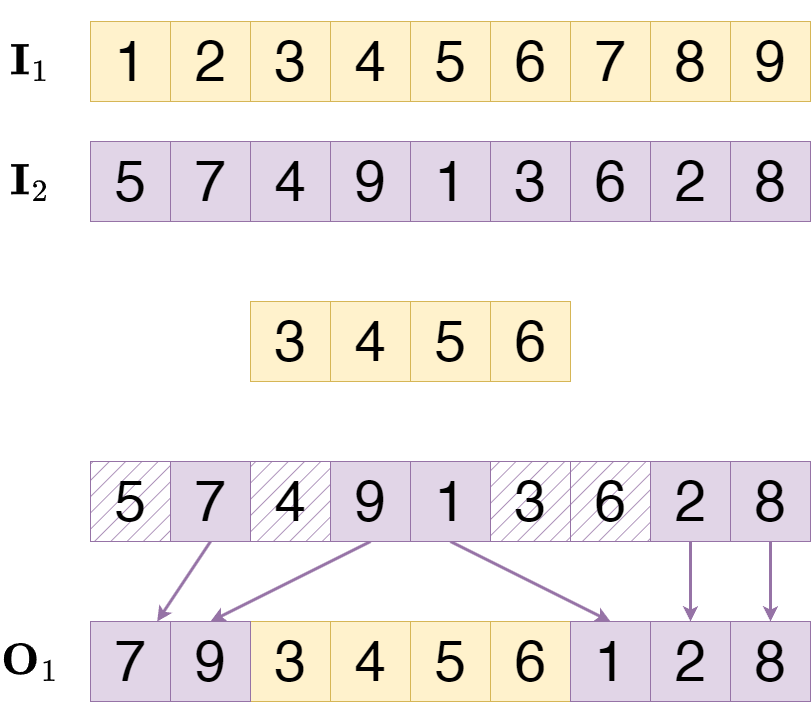
\includegraphics[width=0.33\textwidth]{img/keen/OX.png}
    \caption{Ordered Crossover (OX) operator.}
    \label{fig:keen:op:cx:ox}
  \end{figure}
